
\chapter{Experiments~\label{ch:experiments}}
Experiments were conducted to check if the implemented GNN is able to cope with the tasks presented in the original article~\cite{scarselli2009graph}. For all the experiments the state size was set to 5, the number of hidden neurons in both the $h_{\bm{w}}$ and $g_{\bm{w}}$ networks was set to 5. After some successful trivial experiments, consisting of memorizing a single graph, the proper experiments were conducted. The task chosen for experiments was the \emph{subgraph matching} task. It was chosen, because:
\begin{enumerate}
	\item a similar experiment was conducted by Scarselli et al.~\cite{scarselli2009graph}
	\item the dataset is easy to generate, yet the problem is not trivial
	\item to yield good results, the structure of the graph have to be exploited.
\end{enumerate}

\section{Subgraph matching - data}
The datasets for the subgraph matching task were generated as follows. For a given number of graph nodes, graphs were generated by selecting node labels from $[0..10]$ and connecting each node pair in a graph with an edge probability $\delta$. Then, edges were inserted randomly until the graph became connected. Then, a smaller (connected) subgraph $S$ was inserted to every graph in the dataset. Then, a brute force algorithm was used to locate all copies of the subgraph $S$ in every graph in the dataset. Thus, every graph in the dataset contained at least on copy of the subgraph $S$. Afterwards, a small Gaussian noise with zero mean and standard deviation of $0.25$ was added to all node labels. All graph edges were undirected and thus were transformed to pairs of directed edges prior to processing. No edge labels were used.

Two datasets were generated. One with graph size (number of nodes) equal to 6, the subgraph size equal to 3 and $\delta = 0.8$ (100 graphs, called later the \emph{6-3 dataset}). The second dataset with graph size equal to 14, subgraph size equal to 7 and $\delta = 0.2$ (100 graphs, called later the \emph{14-7 dataset}). A larger $\delta$ was used for the first dataset, as graphs generated with $\delta = 0.2$ were mostly sequences. The first dataset was used to analyze the process of training, while the second one was used for comparison of GNN with a standard FNN classifier.

\begin{figure}[h!]
\begin{center}
	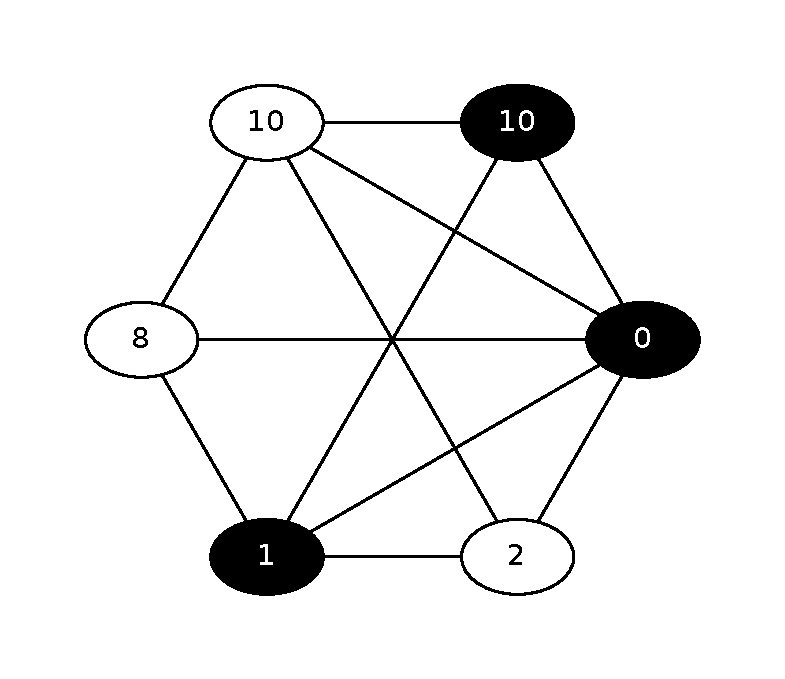
\includegraphics[scale=0.6]{img/g6s3_1.pdf}
	\caption{Sample graph from 6-3 dataset (subgraph in black), before adding noise}
	\label{fig:gnn_g6s3}
\end{center}
\end{figure}

\begin{figure}[h!]
\begin{center}
	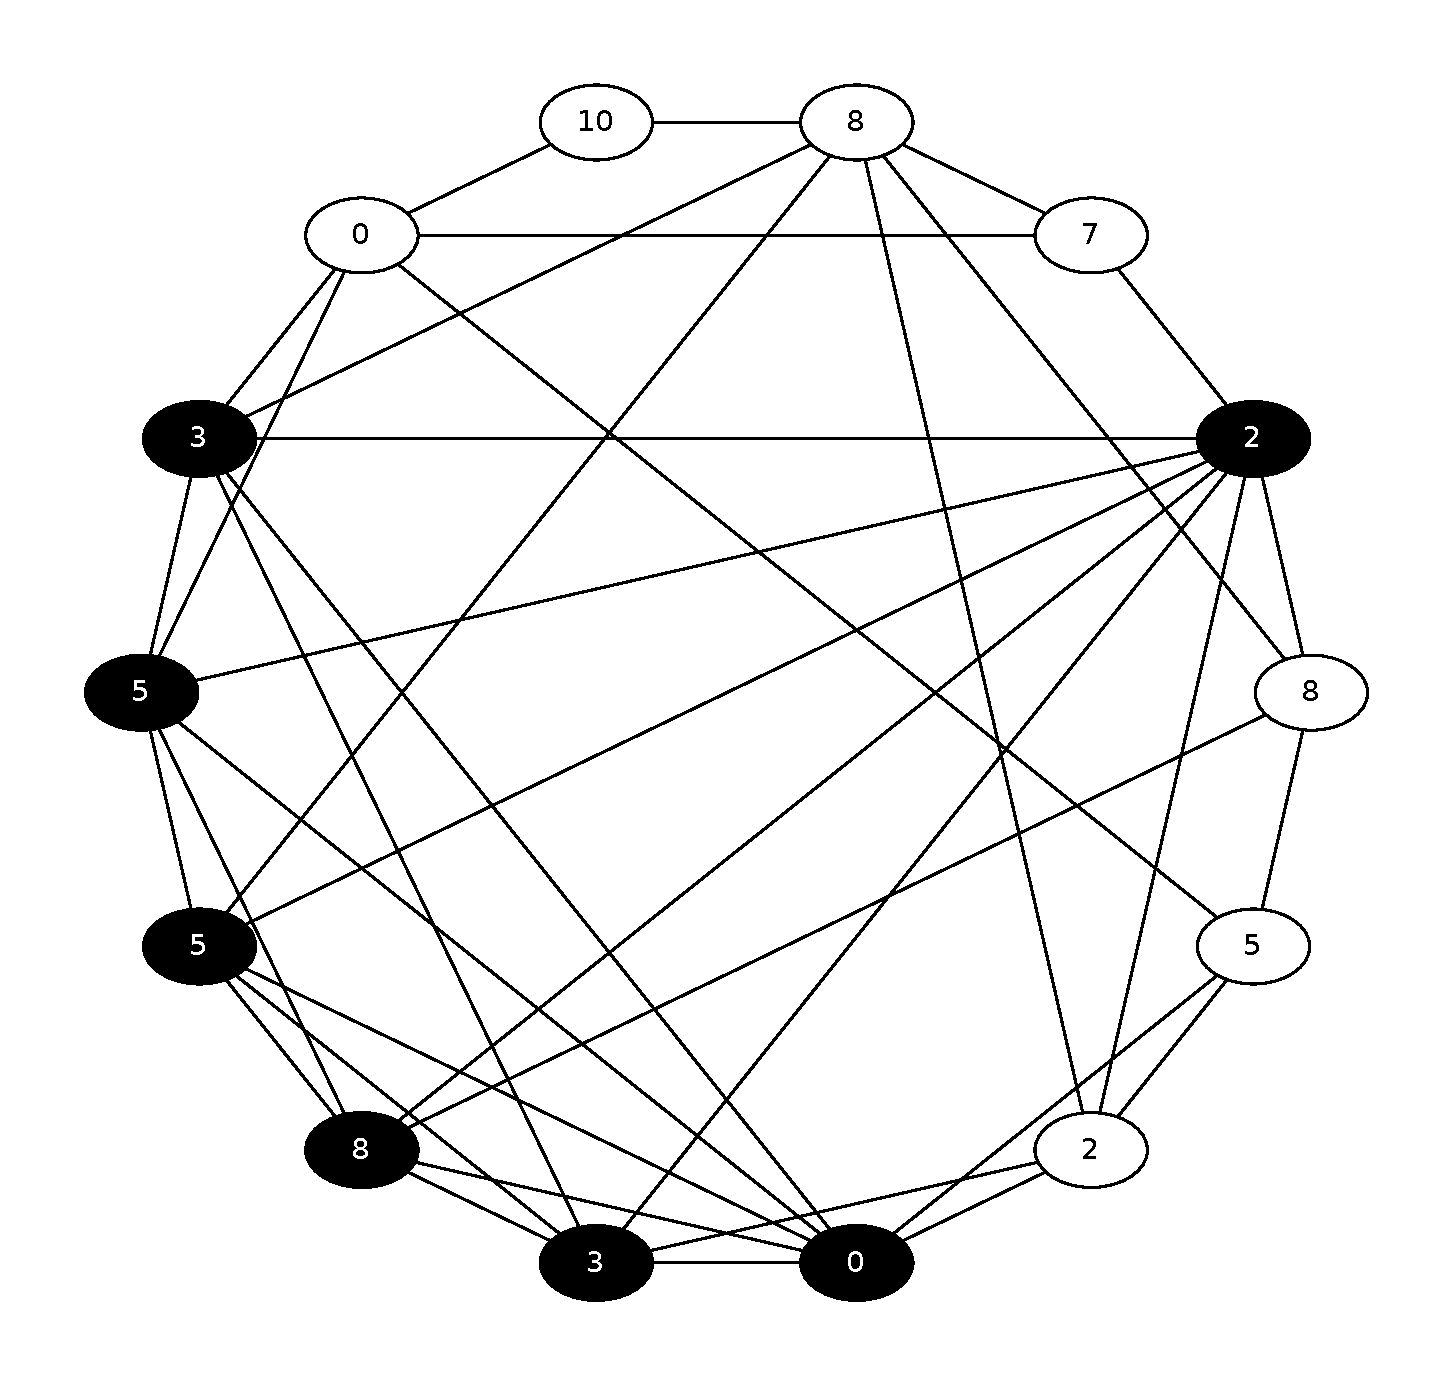
\includegraphics[scale=0.6]{img/g14s7_7.pdf}
	\caption{Sample graph from 14-7 dataset (subgraph in black), before adding noise}
	\label{fig:gnn_g6s3}
\end{center}
\end{figure}

\newpage
\section{Impact of initial weight values on learning}
To test the impact of initial weight values on the process of a GNN training, 9 different sets of weights were tested. For all tested networks, the contraction constant ($\mu$ from Eq.~\ref{eq:gnn_pw}) was set to $0.9$. The training was performed on 10 graphs belonging to the 6-3 dataset. Each GNN network was trained for 50 iterations. As the default error measure used in GNN training is the Mean Square Error, a similar performance measure - RMSE was used for evaluation. Results are presented in Fig.~\ref{fig:gnn_multiple}. Out of 9 networks, only 4 performed well: gnn2, gnn3, gnn5 and gnn7. The gnn5 network yielded the smallest RMSE at the end of training and also presents a remarkably monotonous RMSE slope compared to gnn7. All the other networks didn't improve significantly on the RMSE value, which may suggest that multiple initial sets of weights should be tried for a given dataset to build an efficient classifier.

\begin{figure}[h!]
\begin{center}
	\includegraphics[scale=0.09]{img/rmse_gnn1-9}
	\caption{RMSE for 9 different initial weight sets. $\mu = 0.9$}
	\label{fig:gnn_multiple}
\end{center}
\end{figure}

\newpage
\section{Impact of contraction constant on learning~\label{sec:contraction_constant}}
During the initial experiments, interesting results were obtained for different values of the contraction constant ($\mu$ from Eq.~\ref{eq:gnn_pw}). It seems that for a given learning task exists a minimum value of $\mu$ below which no learning occurs. Some experiments were conducted for the 6-3 dataset using the best networks from Fig.~\ref{fig:gnn_multiple}: the gnn5 and gnn7 network (initial weight values were used). The results for gnn7 are presented in Fig.~\ref{fig:gnn7} and the results for gnn5 are presented in Fig.~\ref{fig:gnn5}. For both networks three different values of $\mu$ were tested: 1.2, 0.9 and 0.6. In both cases it can be observed that no training occurs for $\mu = 0.6$. For these experiments 20 graphs from the 6-3 dataset were used.

\begin{figure}[h!]
\begin{center}
	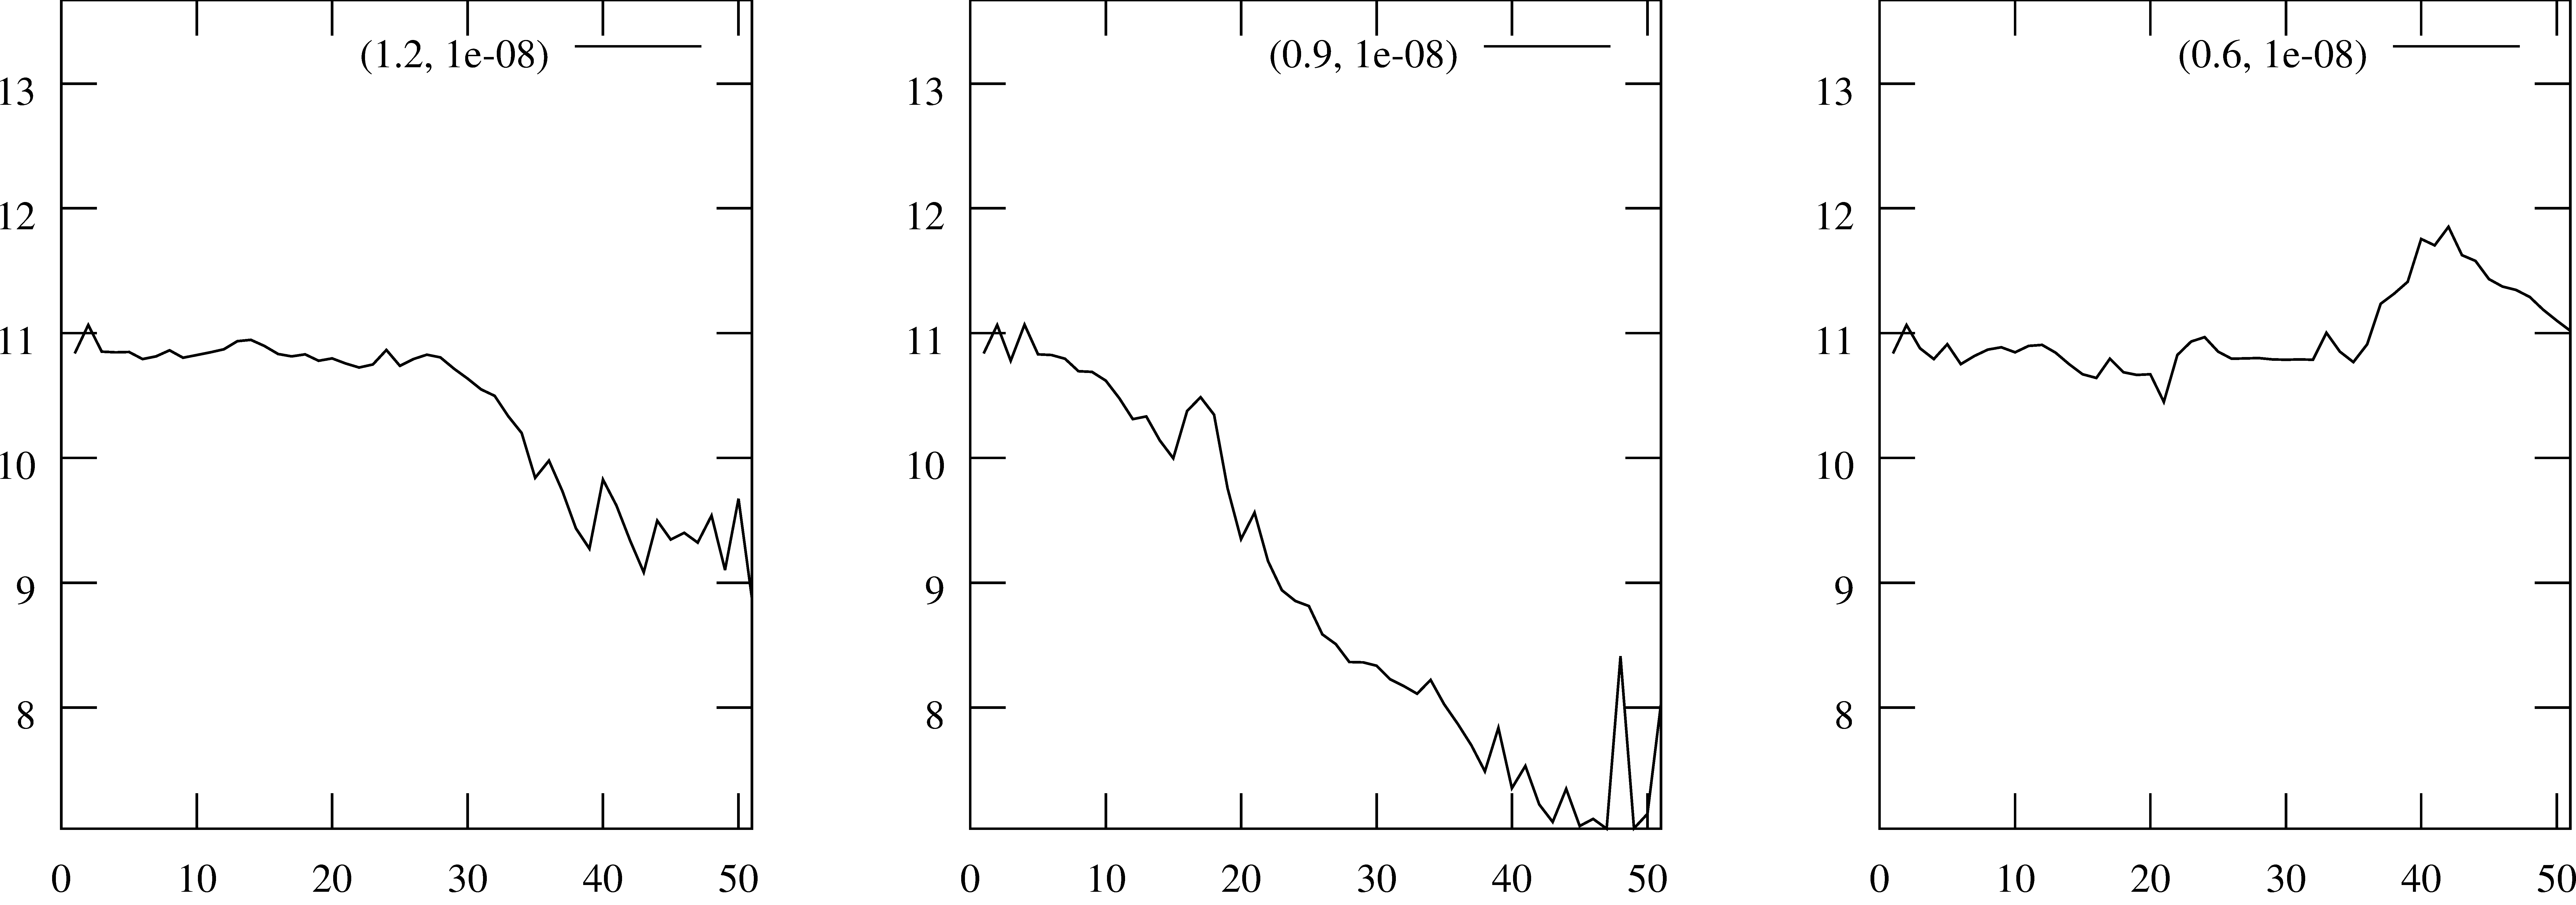
\includegraphics[scale=0.09]{img/rmse_clipped}
	\caption{RMSE for gnn7 with $\mu \in [1.2, 0.9, 0.6]$}
	\label{fig:gnn7}
\end{center}
\end{figure}

\begin{figure}[h!]
\begin{center}
	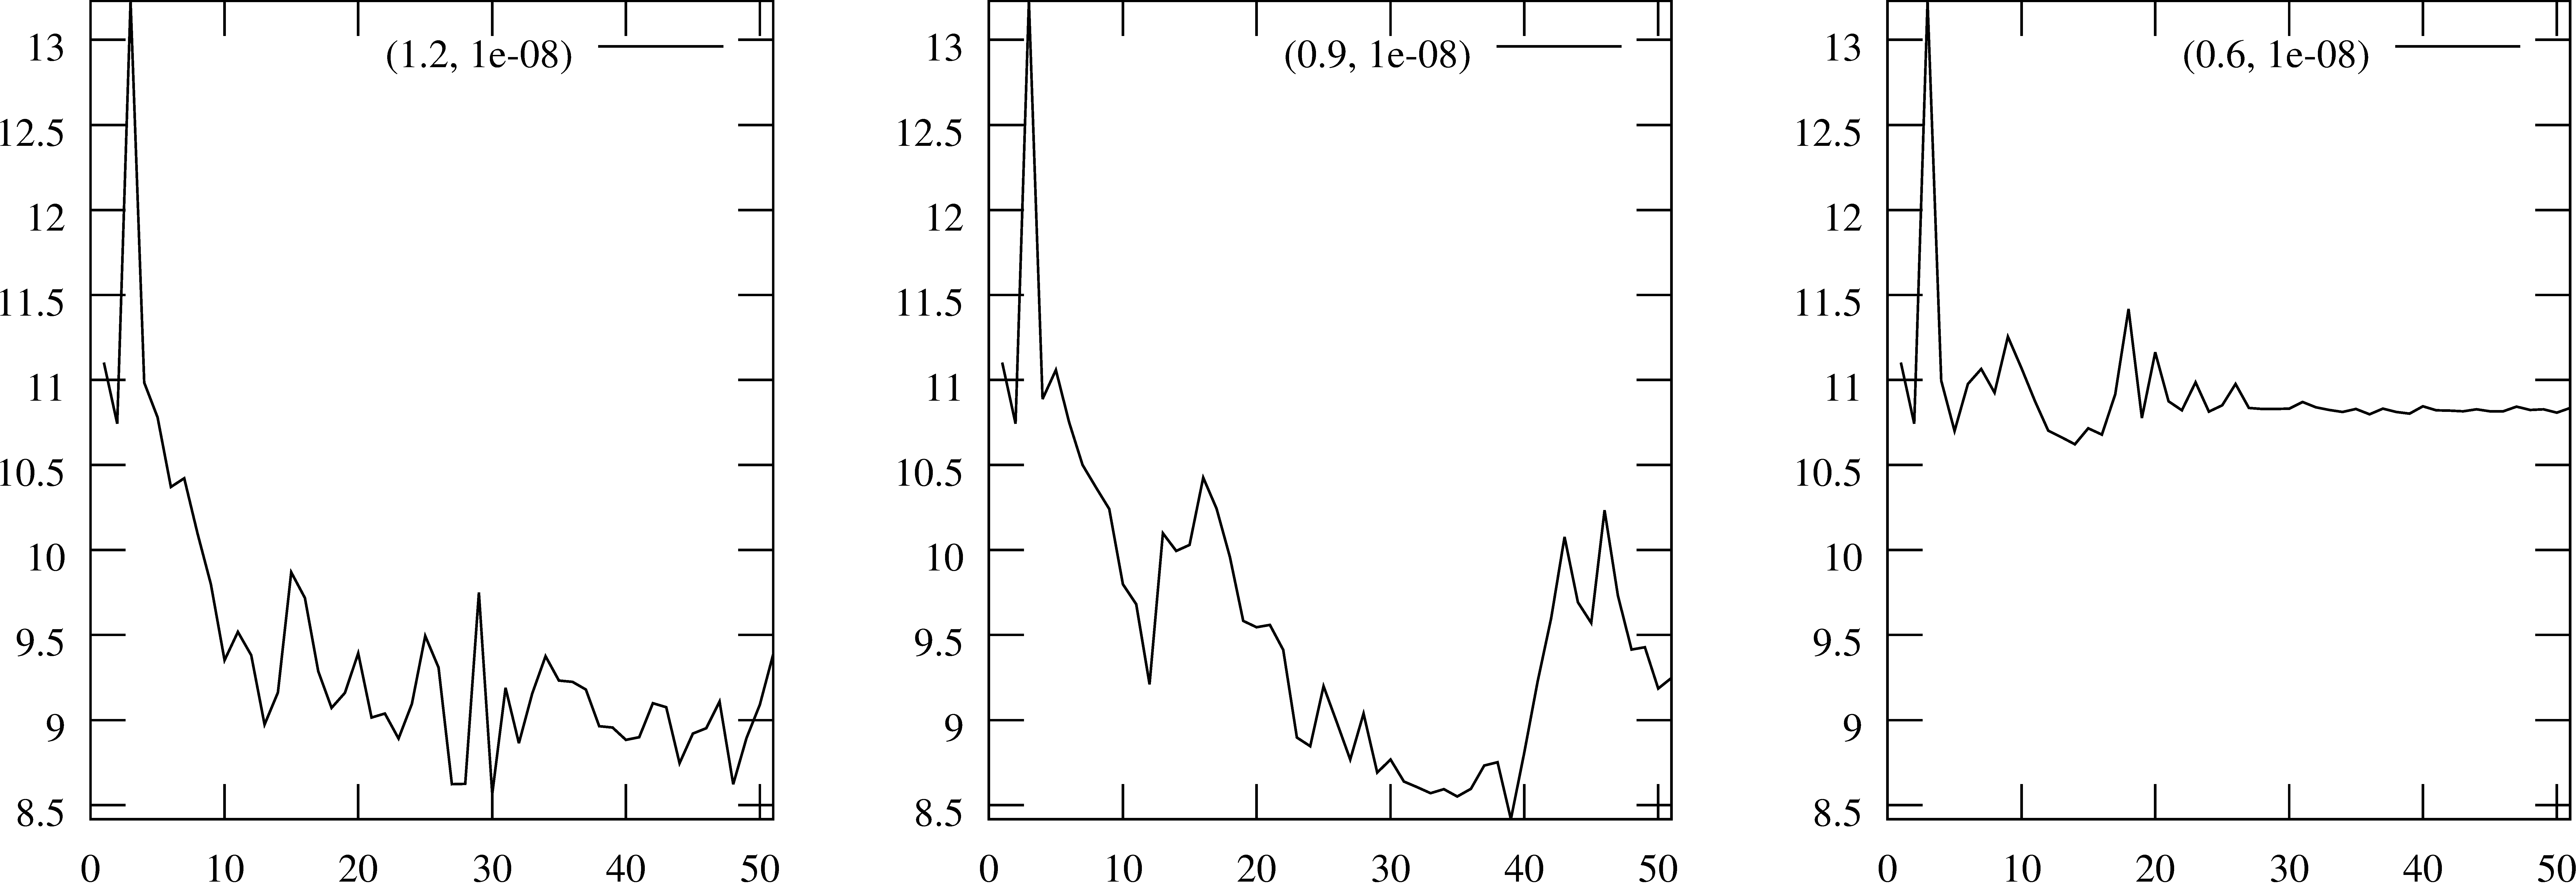
\includegraphics[scale=0.09]{img/rmse1a_clipped}
	\caption{RMSE for gnn5 with $\mu \in [1.2, 0.9, 0.6]$}
	\label{fig:gnn5}
\end{center}
\end{figure}

A closer look on the process of learning may shed some light on the reasons behind the lack of learning. In Fig.~\ref{fig:gnn5_09} the process of learning of gnn5 with $\mu = 0.9$ is presented. In Fig.~\ref{fig:gnn5_06} the same network gnn5 was trained with $\mu = 0.6$. The different values shown are: \emph{nForward} - number of \emph{Forward} (state building) iterations, \emph{nBackward} - number of \emph{Backward} (error accumulation) iterations, \emph{penalty} - set to 1 if any weight was penalized, \emph{de/dw influence} - percent of combined weight updates that had the same sign as~$\frac{\partial e}{\partial w}$ (before passing to RPROP algorithm), \emph{dp/dw influence} - percent of combined weight updates that had the same sign as~$\frac{\partial p}{\partial w}$. Some interesting features of the GNN model learning schema can be observed. In the case of $\mu = 0.9$ the number of \emph{Forward} steps reached the maximum a couple of times, which presumably means that at that time the $F_{\bm{w}}$ ceased being a contraction map. The penalty was imposed mostly for short periods of time and only at one moment caused the $\frac{\partial e}{\partial w}$ influence to drop below 50\%. This strategy yielded good results - the imposed penalty reduced the number of \emph{Forward} steps and the RMSE was successfully reduced.

\begin{figure}[h!]
\begin{center}
	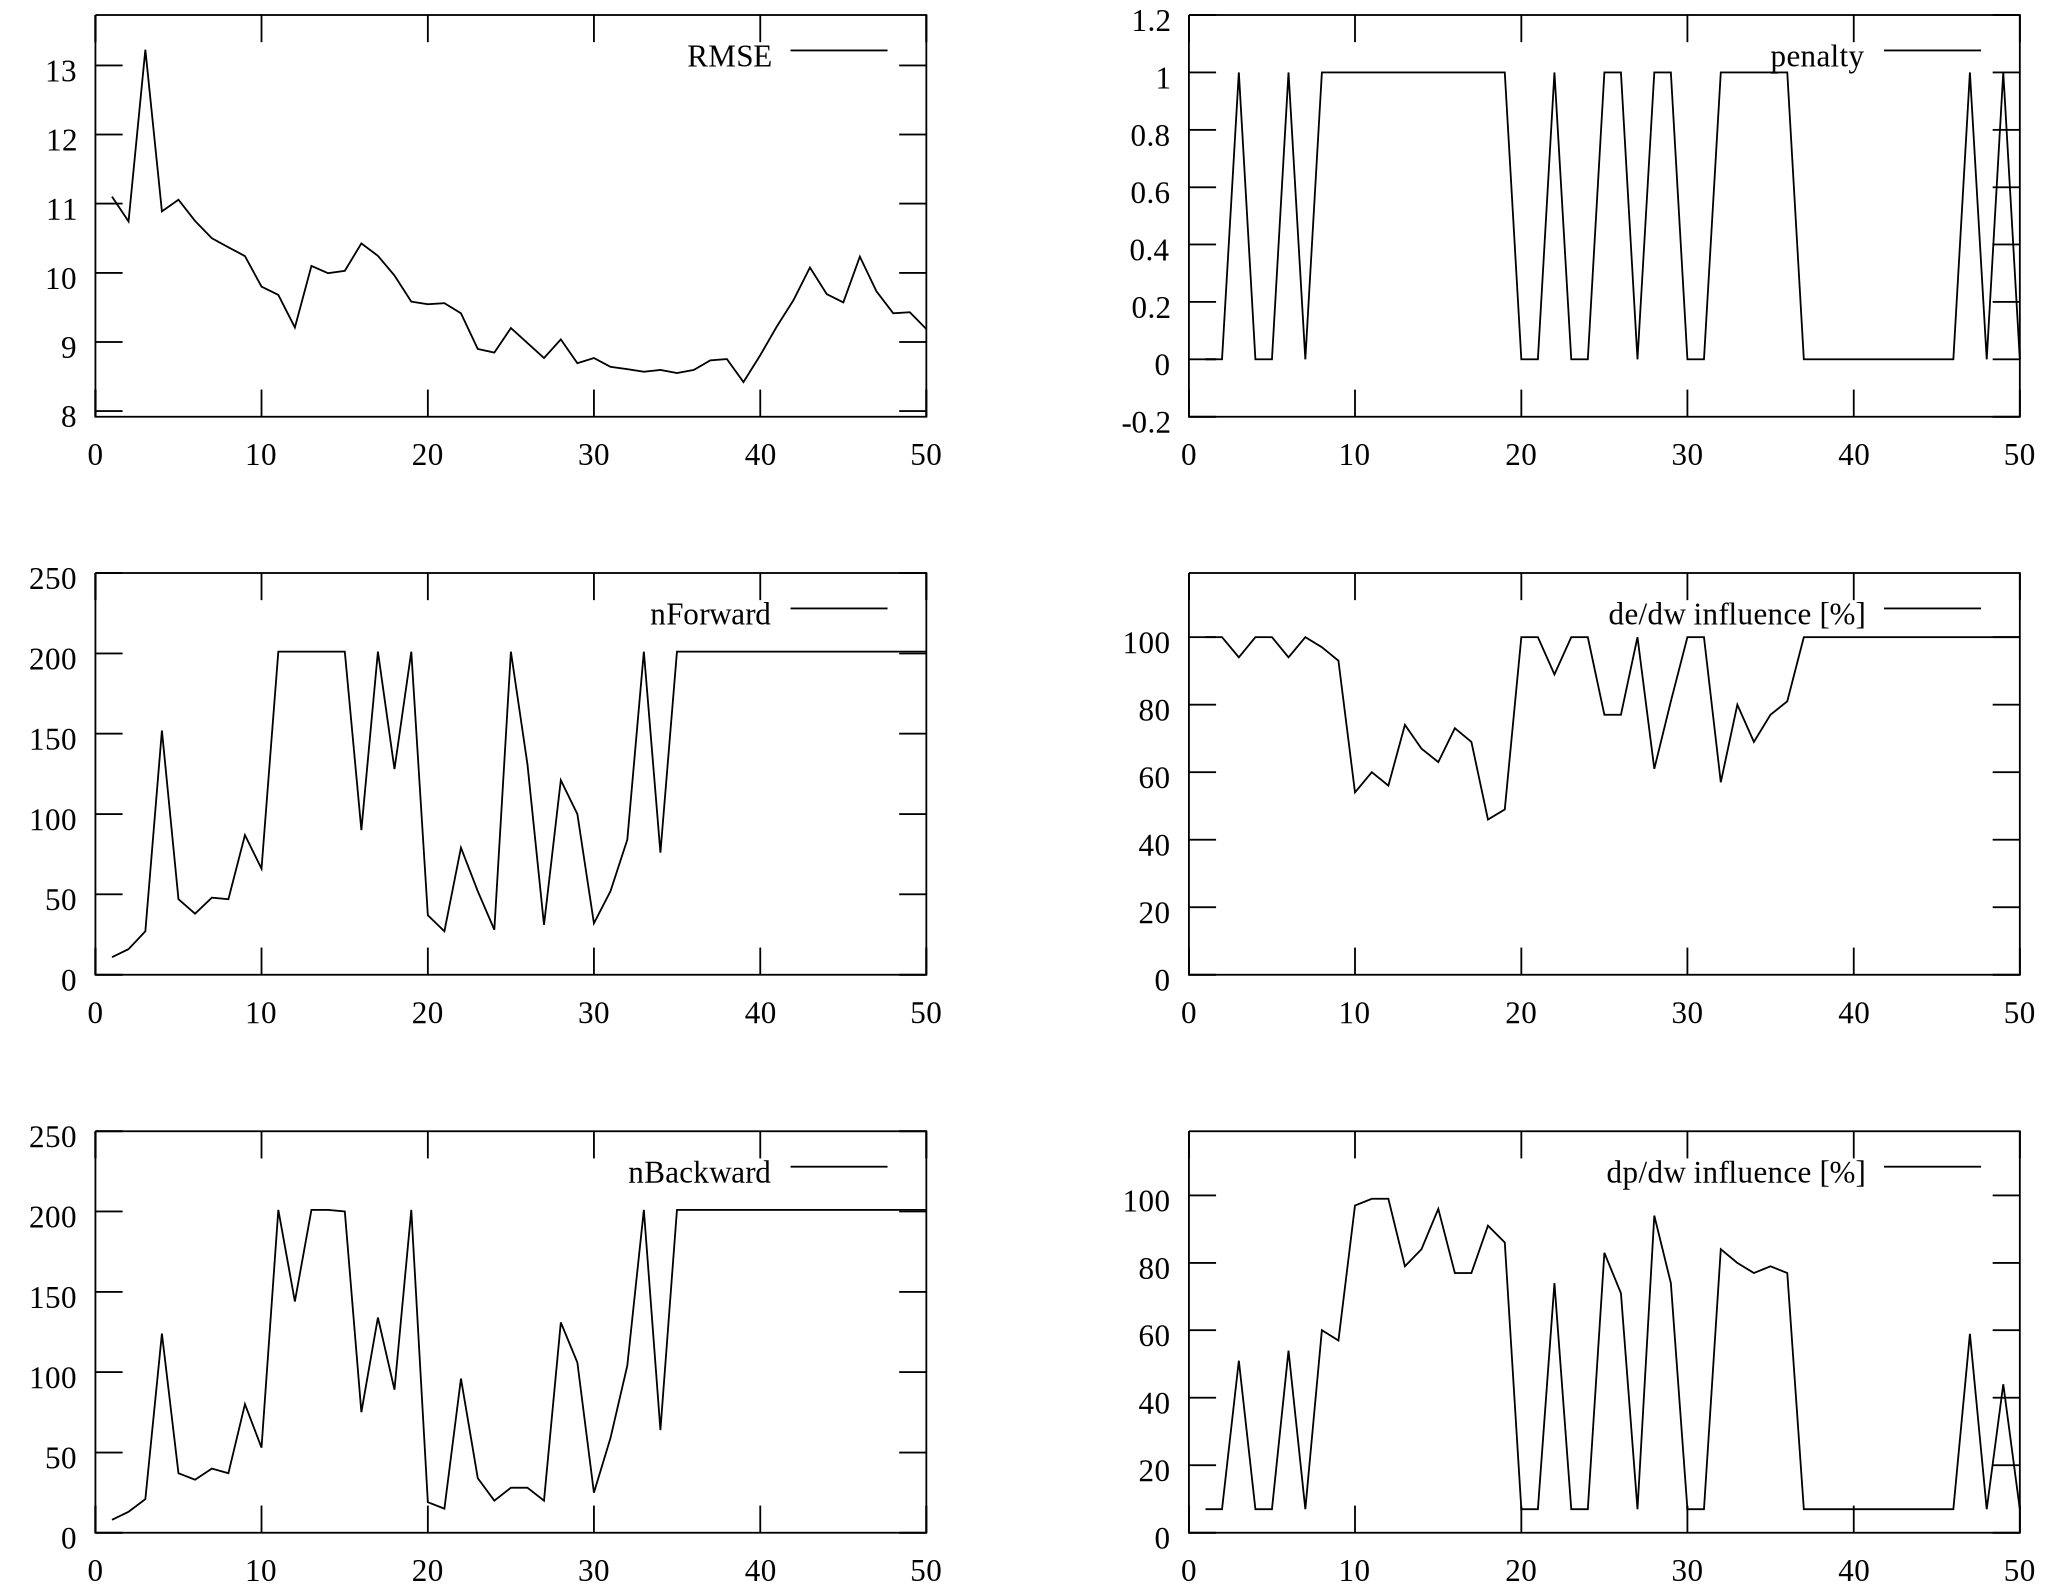
\includegraphics[scale=0.09]{img/gnn1_2}
	\caption{gnn5 performance with $\mu = 0.9$ for 20 graphs}
	\label{fig:gnn5_09}
\end{center}
\end{figure}

A different situation is shown for $\mu = 0.6$. Because of a low $\mu$ value, the penalty was imposed eagerly and was larger than in the previous case (the impact of the $\mu$ value was described in section~\ref{sec:contraction}). It was imposed even when the number of \emph{Forward} steps was below the maximum, that is when $F_{\bm{w}}$ was still a contraction map. Large values of the penalty caused a huge decrease of the $\frac{\partial e}{\partial w}$ term influence, which made any learning impossible.

\begin{figure}[h!]
\begin{center}
	\includegraphics[scale=0.09]{img/gnn1_3}
	\caption{gnn5 performance with $\mu = 0.6$ for 20 graphs}
	\label{fig:gnn5_06}
\end{center}
\end{figure}

\newpage
Another interesting case is presented in Fig.~\ref{fig:gnn5_09_10}: the learning process of gnn5 on 10 graphs with $\mu = 0.9$. It can be observed that even as the number of \emph{Forward} steps reached in peaks the maximum value, the $F_{\bm{w}}$ function remained a contraction map. A large enough $\mu$ prevented the penalty from being imposed, which enabled the GNN model to train both computation units without any disturbance. The result is a monotonously decreasing RMSE slope, which could be previously observed in Fig.~\ref{fig:gnn_multiple}. It can be concluded, that the most important aspect of building a GNN model is to provide an efficient way to make $F_{\bm{w}}$ a contraction map as fast as possible, so as to provide as much time as possible for undisturbed learning.

\newpage
\begin{figure}[h!]
\begin{center}
	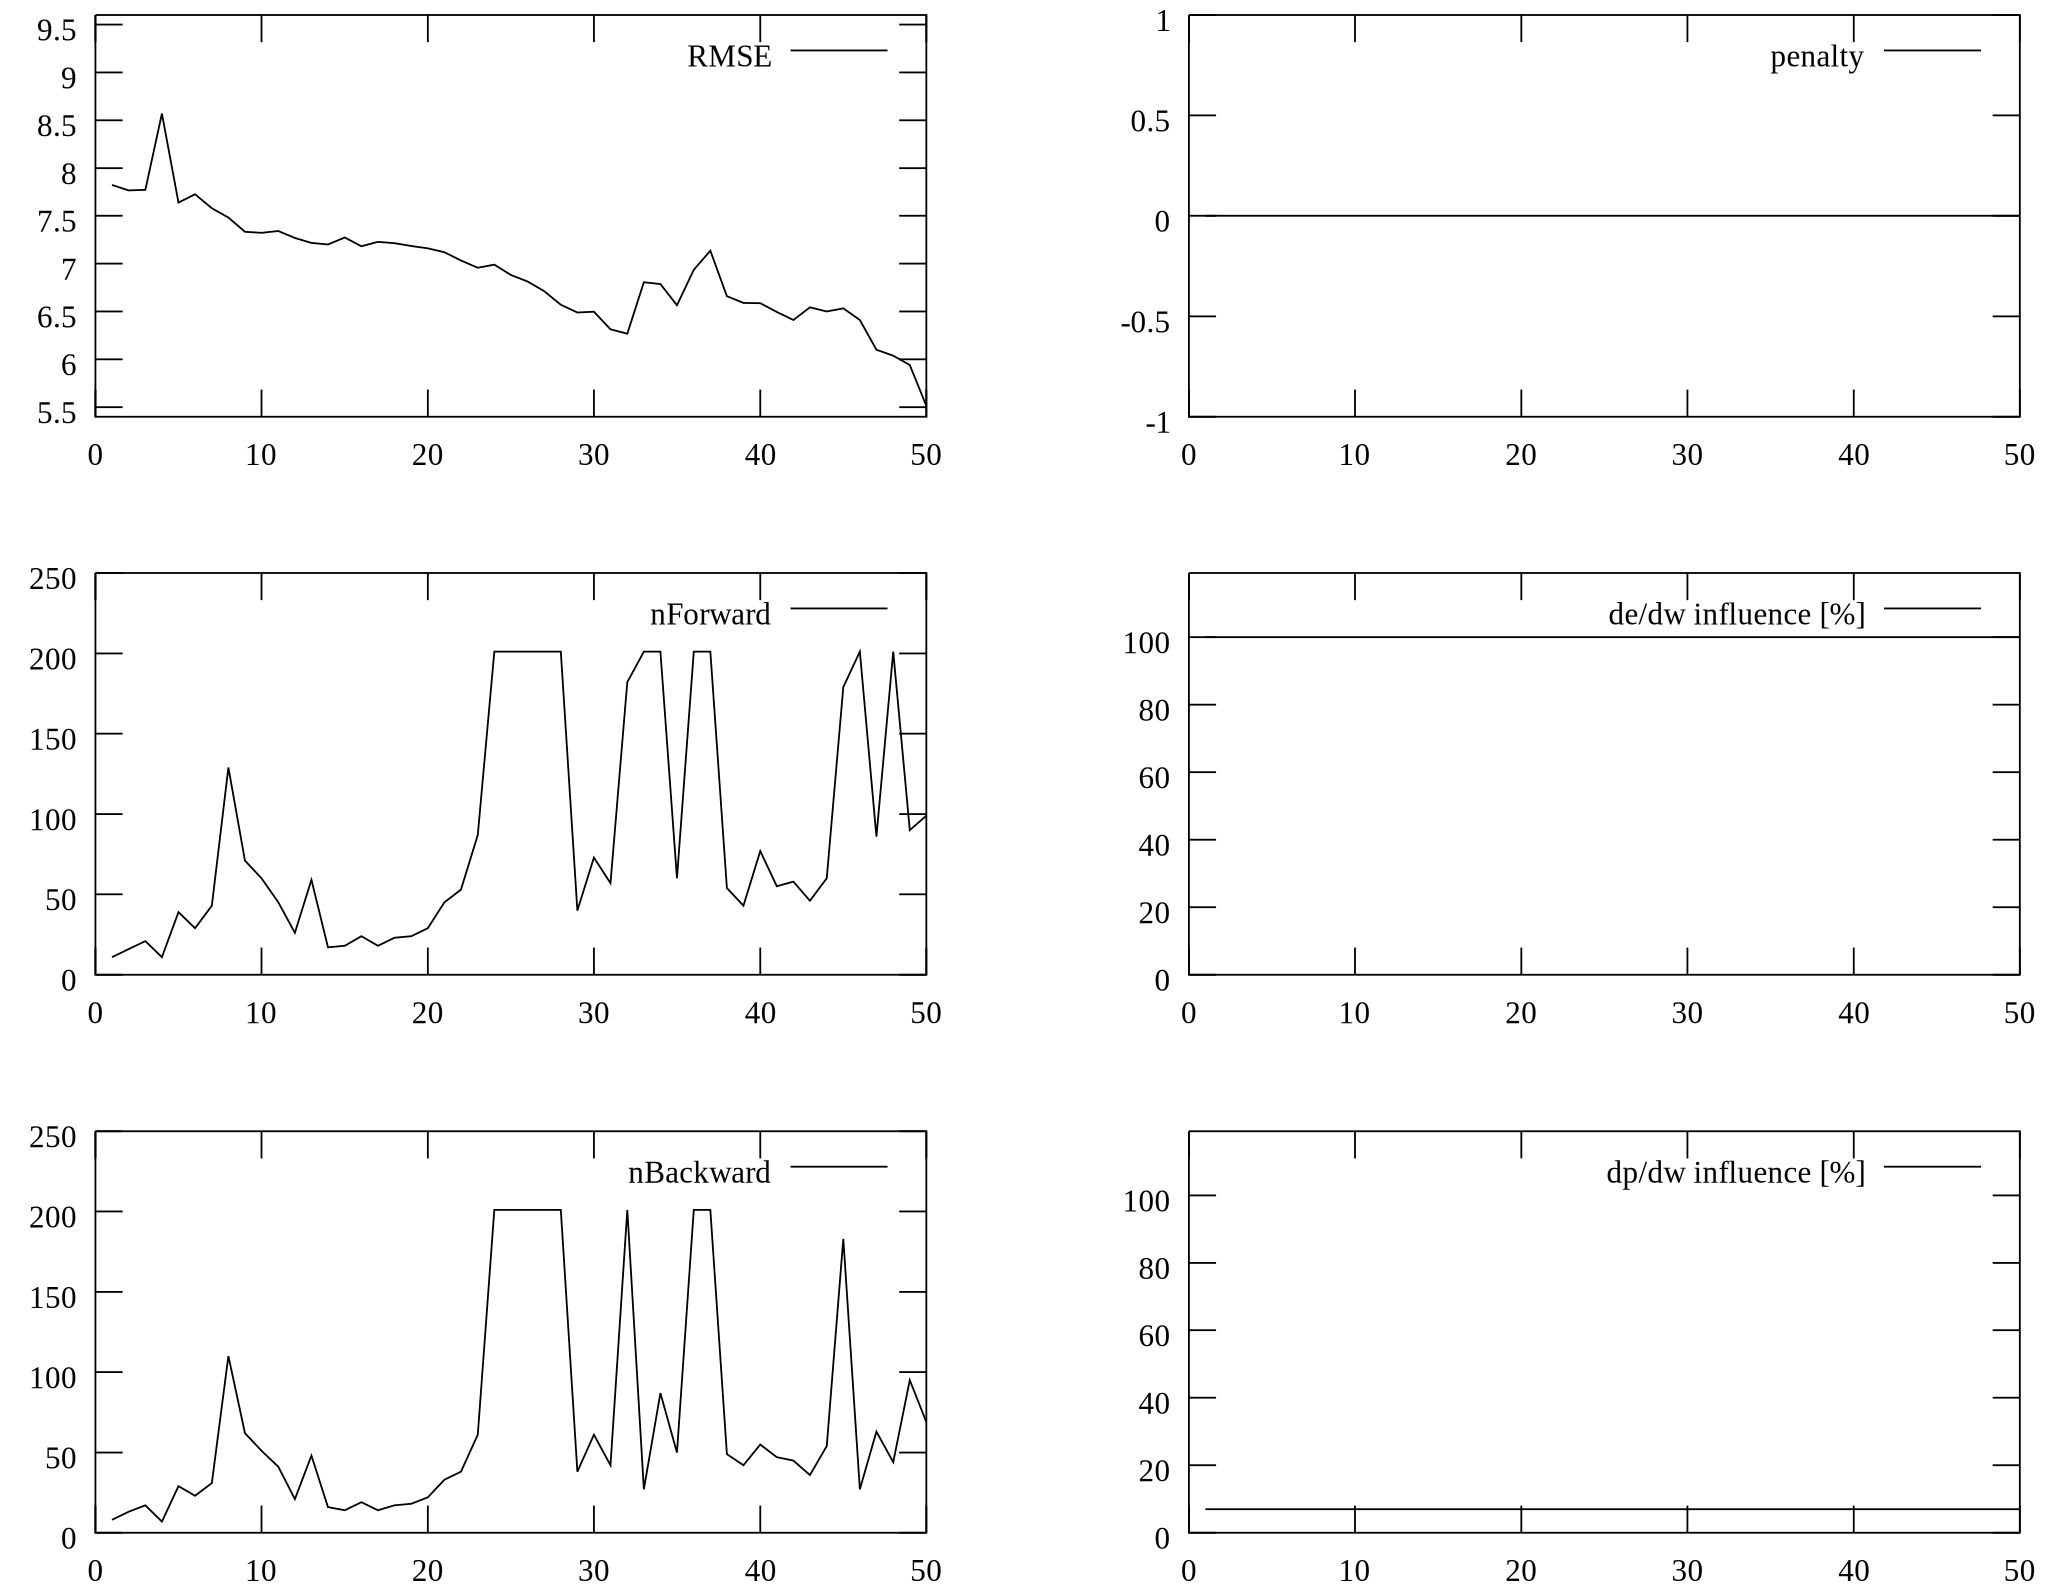
\includegraphics[scale=0.09]{img/gnn5}
	\caption{gnn5 performance with $\mu = 0.9$ for 10 graphs}
	\label{fig:gnn5_09_10}
\end{center}
\end{figure}

\newpage
\section{Cross-validation results}
To compare the performance of the implemented GNN model with a standard FNN, the following subgraph matching experiment was conducted. 5-fold cross-validation was performed on all 100 graphs from the 14-7 dataset. A random GNN was generated. It was trained with a contraction constant $\mu = 0.9$ for 50 iterations for each fold. To provide good FNN results, 10 three-layer FNNs with 20 hidden $tanh$ neurons were evaluated and the one with best mean accuracy was selected. The results are presented in Table~\ref{tab:crossmean} and~\ref{tab:crossstd}. The GNN classifier outperformed the FNN by more than 15\%. This is due to the fact, that the FNN classifier could make predictions only by analyzing node labels, while the GNN classifier exploited correctly the graph topology.

These results can be better understood by analyzing the classified dataset. The 100 processed graphs consisted in total of 1400 nodes. Amongst these nodes, 1031 had node labels matching the subgraph node labels. Amongst these 1031 nodes only 702 actually belonged to the subgraph. Thus, 329 nodes, 23.5\% of all the nodes would probably be classified as false positives by a classifier taking into consideration only node labels. This hypothesis corresponds quite well with the results presented.

\begin{table}[h!]
	\begin{center}
	\begin{tabular}{llll}
	\toprule
	& accuracy & precision & recall \\
	\midrule
	FNN - tr &	75\% &  68\% &  93\% \\
	FNN - tst &	74\% &  68\% &  93\% \\
	GNN - tr &	91\% &  87\% &  97\% \\
	GNN - tst &	91\% &  86\% &  97\% \\
	\bottomrule
	\end{tabular}
	\caption{Mean values on training and test sets}
	\label{tab:crossmean}
	\end{center}
\end{table}

\begin{table}[h!]
	\begin{center}
	\begin{tabular}{llll}
	\toprule
	& accuracy & precision & recall \\
	\midrule
	FNN - tr &	0.68\% &  0.82\% &  1.43\% \\
	FNN - tst &	3.20\% &  2.89\% &  1.85\% \\
	GNN - tr &	1.62\% &  1.71\% &  2.07\% \\
	GNN - tst &	3.06\% &  3.70\% &  1.39\% \\
	\bottomrule
	\end{tabular}
	\caption{Standard deviations on training and test sets}
	\label{tab:crossstd}
	\end{center}
\end{table}
